\newpage

\section{Soft constraints}

I vincoli soft permettono di associare un \textbf{livello di preferenza} a
ciascun assegnamento di valori per una tupla.

Questo implica che non ci sono più solo due livelli di soddisfacibilità
(0 e 1), ma molti altri\dots\\

\textbf{Esempio}: si vuole decidere cosa mangiare in un ristorante, dato
un certo menù. Si possono avere delle preferenze sui singoli piatti o
bevande e sulla loro combinazione. Si cerca il pasto che massimizzi
la preferenza di un cliente.

Un \textbf{vincolo soft} è simile a un vincolo classico, dove ciascun
assegnamento di valori alle variabili è associato a un valore di
preferenza (appartenente a un insieme parzialmente ordinato).

La figura \ref{fig:soft} mostra un vincolo soft per il problema del
ristorante.

\begin{figure}[H]
\centering
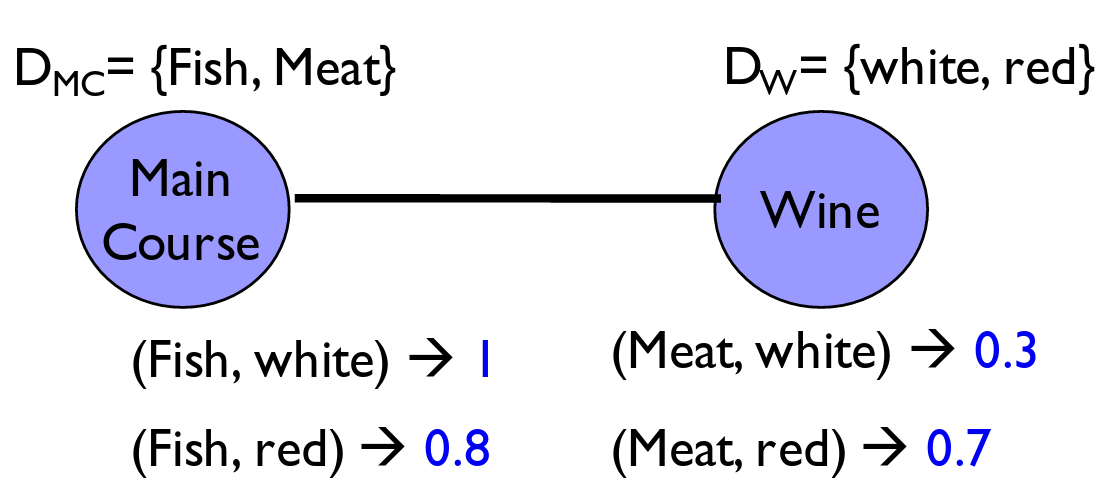
\includegraphics[width=0.5\textwidth]{soft}
\caption{Esempio di vincolo soft per il problema del ristorante}
\label{fig:soft}
\end{figure}

L'insieme parzialmente ordinato dei valori di preferenza ha 2 operazioni e
questo lo rende simile a un semianello. Si basa sulla struttura
\textbf{c-semianello}.

\subsection{Formalismo dei c-semianelli}

Sia $<A, +, *, 0, 1>$ un semianello:

\begin{itemize}
 \item A è l'insieme dei valori di preferenza
 \item + è l'operazione di proiezione
 \item * è l'operazione di combinazione
 \item 0 è l'elemento che corrisponde al peggior valore di preferenza $0 \in A$
 \item 1 è l'elemento che corrisponde al miglior valore di preferenza $1 \in A$
\end{itemize}

Un problema CSP soft consiste in un insieme di vincoli soft su un insieme di
variabili basate su uno specifico c-semianello.

Una soluzione consiste come sempre in un assegnamento completo di valori alle
variabili.

Una soluzione, inoltre, possiede un valore di preferenza, combinando le
preferenze dei singoli valori.

Un \textbf{c-semianello fuzzy} ha valori di A in un insieme continuo [0,1]:
$<A = [0,1], + = max, * = min, 0 = 0, 1 = 1>$. La combinazione fra due o
più valori in questo c-semianello avviene prendendo il valore minimo,
la proiezione avviene prendendo il valore massimo.

\begin{figure}[H]
\centering
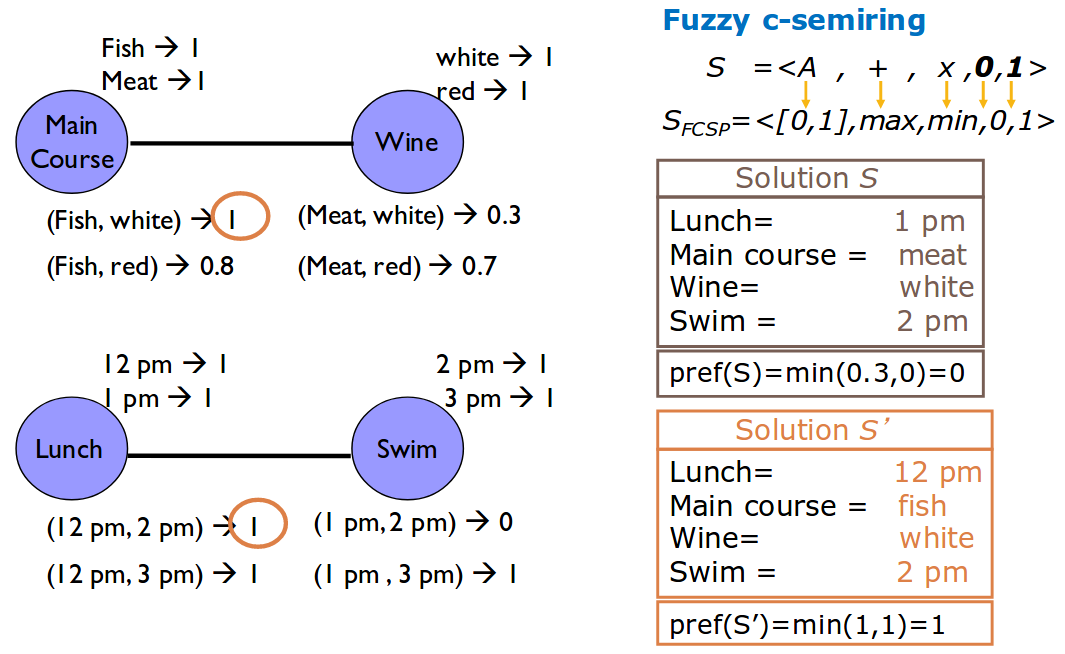
\includegraphics[width=0.8\textwidth]{esempioFuzzy}
\caption{Esempio di vincoli soft con c-semianello fuzzy}
\label{fig:esempioFuzzy}
\end{figure}

In figura \ref{fig:esempioFuzzy} è riportato l'esempio di un problema
csp fuzzy (FCSP). Ci sono i vincoli soft con le preferenze associate a
ciascun assegnamento sulla sinistra e due soluzioni possibili a destra.

Per determinare quale delle due soluzioni è la migliore, si devono trovare
i loro valori di preferenza, combinando i singoli valori degli assegnamenti
in base ai vincoli soft. In questo esempio la seconda soluzione $S'$ è
migliore della prima.

Un \textbf{c-semianello pesato} ha valori nell'insieme dei numeri naturali.
La combinazione dei valori di preferenza avviene prendendo la loro somma.
È utile in tutti i contesti in cui sono coinvolti dei costi (occorre
minimizzare la loro somma).

Un soft CSP induce un ordine sulle soluzioni, dall'ordine del c-semianello
(che può ossere totale o parziale).

L'idea generale è quella di usare un c-semianello per ogni criterio di
ordinamento, attraverso i \textbf{multi-criteria problems}.

Dati n c-semianelli, si può costruire il c-semianello che li contiene
tutti:
$<<A_1,...,A_n>, +, *, <0_1,...,0_n>,<I_1,...,I_n>>$.

Esempio: si vuole scegliere che strada percorrere per andare da una città
X a una città Y. Ogni pezzettino di strada ha associato un costo e una
preferenza.
Questo contesto è adatto per un multi-criteria problems: da un lato si
vuole minimizzare la somma dei costi e dall'altro si vuole massimizzare
la preferenza. Si usano due c-semianelli: quello pesato e quello fuzzy.

\subsection{Operazioni fondamentali con i vincoli soft}

\begin{itemize}
 \item \textbf{Proiezione}: elimina una o più variabili da un vincolo
ottenendo un nuovo vincolo soft e preserva tutte le informazioni delle
rimanenti.
 \item \textbf{Combinazione}: combina due o più vincoli soft in uno
nuovo sintetizzando le informazioni di quelli originali.
\end{itemize}

\textbf{Esempio di proiezione} - si vuole \textbf{eliminare la variabile
``Wine''} dal seguente vincolo fuzzy:

\begin{figure}[H]
\centering
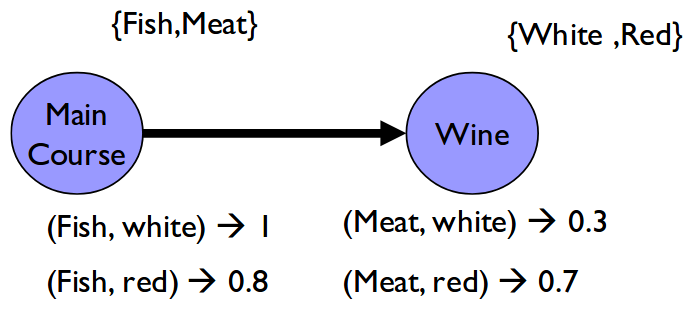
\includegraphics[width=0.45\textwidth]{proj1}
\caption{Eliminare la variabile ``Wine'' dal vincolo fuzzy}
\label{fig:proj1}
\end{figure}

La situazione iniziale è $c=<f,\{mc,w\}>$, dove f è la funzione che
associa una tupla/assegnamento a un valore di preferenza.

Si vuole ottenere il vincolo ristretto alla variabile mc: $c|_{mc}$.

Si considerano tutti i valori di mc e si usa l'operatore di proiezione +
su tutte le tuple con uno stesso valore di mc, dopo aver ricavato
il valore di preferenza della tupla (in questo esempio si applica + su
tutte le tuple che contengono fish e su tutte quelle che contengono meat).

\begin{figure}[H]
\centering
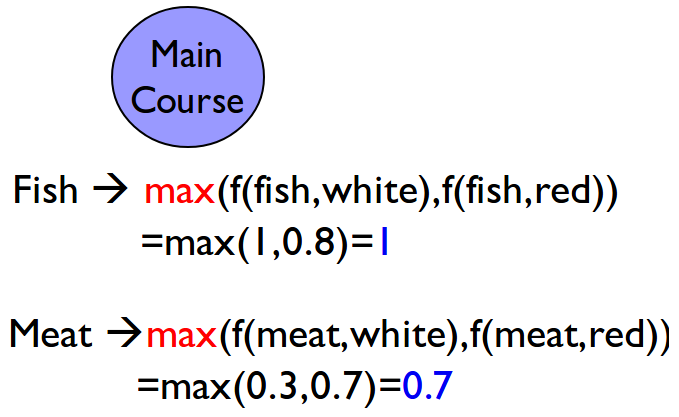
\includegraphics[width=0.45\textwidth]{proj2}
\caption{Vincolo fuzzy che preserva le informazioni del precedente, eliminando
la variabile ``Wine''}
\label{fig:proj2}
\end{figure}

\textbf{Esempio di combinazione} - si vogliono riunire i tre seguenti vincoli
fuzzy che rappresentano le preferenze sulle componenti di un PC:

\begin{figure}[H]
\centering
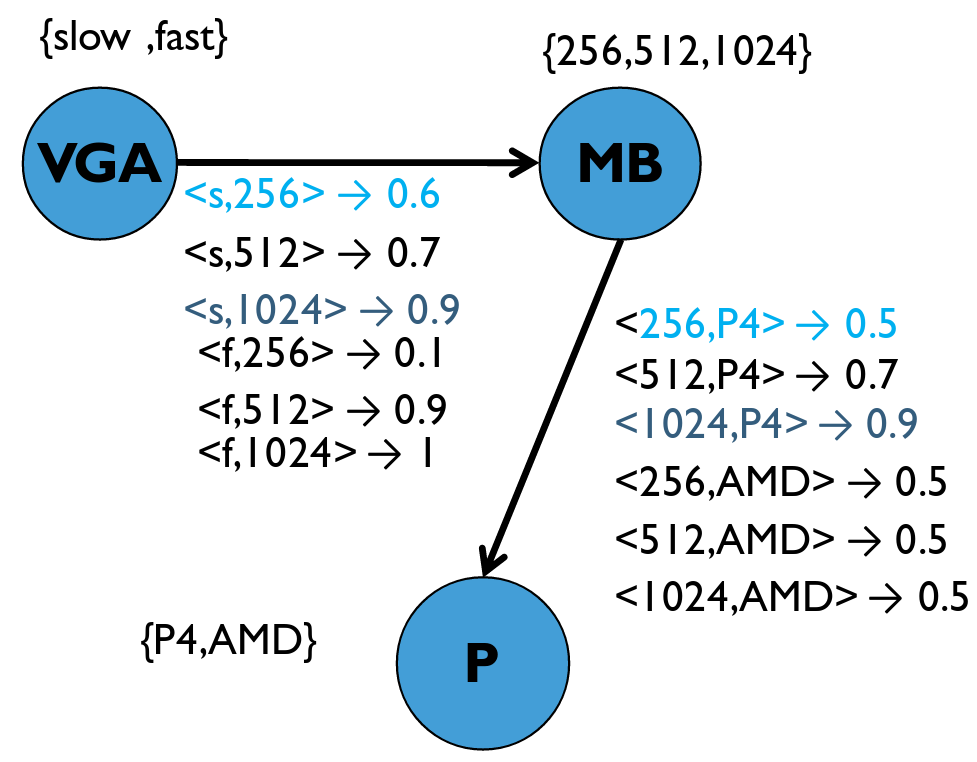
\includegraphics[width=0.45\textwidth]{comb1}
\caption{I vincoli fuzzy da combinare}
\label{fig:comb1}
\end{figure}

Occorre applicare l'operatore di combinazione alle tuple dei vincoli
che si vogliono unire (dopo aver ricavato il loro valore di preferenza).
Le tuple non si possono combinare a caso, se c'è una variabile legata
da più di un vincolo allora occorre combinare le tuple che hanno valori
uguali per la variabile in comune... nell'esempio questa variabile è MB.

\begin{figure}[H]
\centering
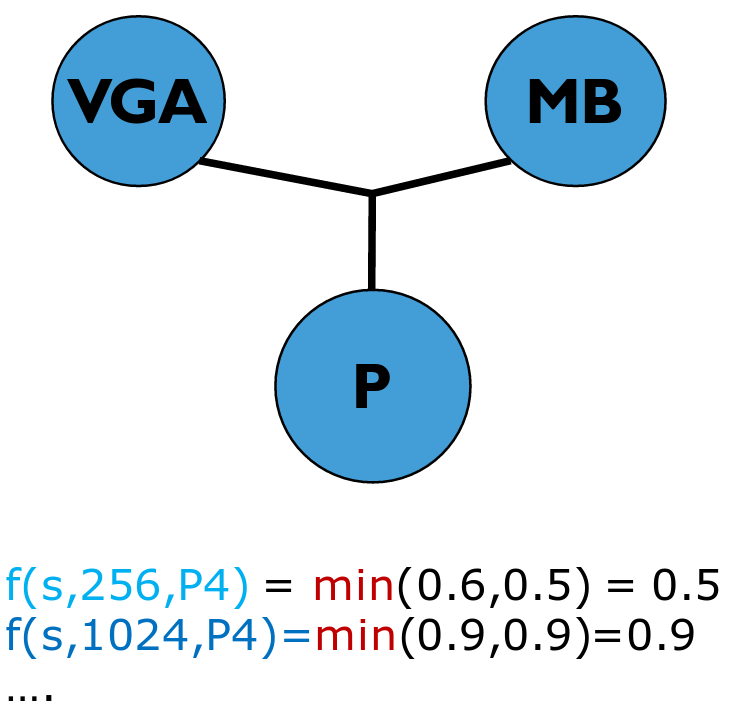
\includegraphics[width=0.4\textwidth]{comb2}
\caption{Vincolo fuzzy che combina i 3 precedenti}
\label{fig:comb2}
\end{figure}

\subsection{Esercizio}

Consider the three fuzzy constraints shown in the figure below.
Draw the constraint which is obtained combining them.

\begin{figure}[H]
\centering
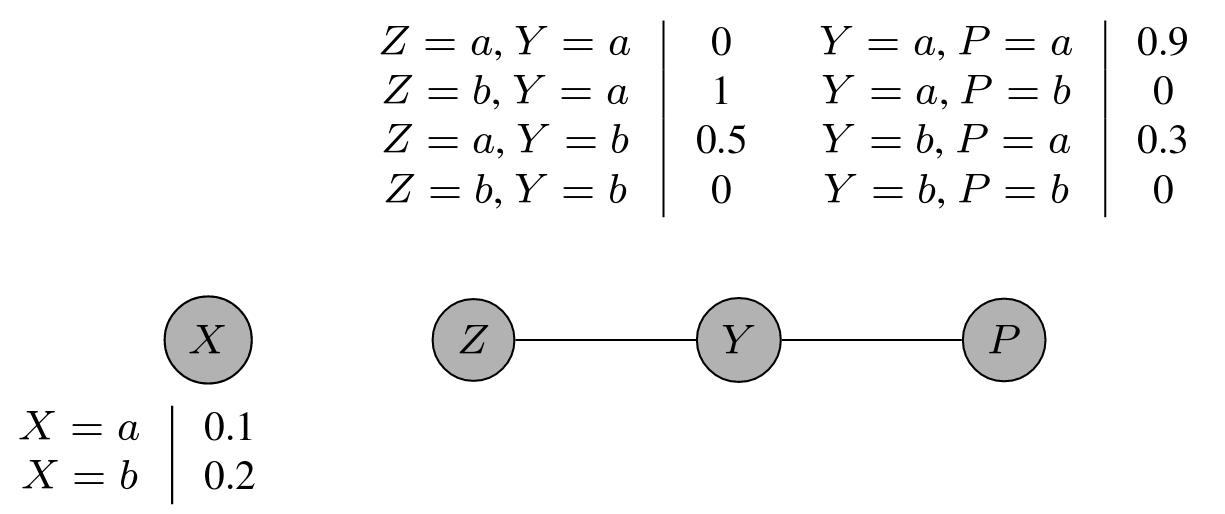
\includegraphics[width=0.65\textwidth]{softEx}
\caption{Esercizio di combinazione}
\label{fig:comb2}
\end{figure}

<X = a, Z = a, Y = a, P = a> $\rightarrow$ min(0.1, 0, 0.9) = 0

<X = a, Z = a, Y = a, P = b> $\rightarrow$ min(0.1, 0, 0) = 0

<X = a, Z = b, Y = a, P = a> $\rightarrow$ min(0.1, 1, 0.9) = 0.1

<X = a, Z = b, Y = a, P = b> $\rightarrow$ min(0.1, 1, 0) = 0

<X = a, Z = a, Y = b, P = a> $\rightarrow$ min(0.1, 0.5, 0.3) = 0.1

<X = a, Z = a, Y = b, P = b> $\rightarrow$ min(0.1, 0.5, 0) = 0

<X = a, Z = b, Y = b, P = a> $\rightarrow$ min(0.1, 0, 0.3) = 0

<X = a, Z = b, Y = b, P = b> $\rightarrow$ min(0.1, 0, 0) = 0\\

E ora si ripetono tutte le combinazioni con X = b\dots\\

<X = b, Z = a, Y = a, P = a> $\rightarrow$ min(0.2, 0, 0.9) = 0

<X = b, Z = a, Y = a, P = b> $\rightarrow$ min(0.2, 0, 0) = 0

<X = b, Z = b, Y = a, P = a> $\rightarrow$ min(0.2, 1, 0.9) = 0.2

<X = b, Z = b, Y = a, P = b> $\rightarrow$ min(0.2, 1, 0) = 0

<X = b, Z = a, Y = b, P = a> $\rightarrow$ min(0.2, 0.5, 0.3) = 0.2

<X = b, Z = a, Y = b, P = b> $\rightarrow$ min(0.2, 0.5, 0) = 0

<X = b, Z = b, Y = b, P = a> $\rightarrow$ min(0.2, 0, 0.3) = 0

<X = b, Z = b, Y = b, P = b> $\rightarrow$ min(0.2, 0, 0) = 0

Il vincolo risultante è:

\begin{figure}[H]
\centering
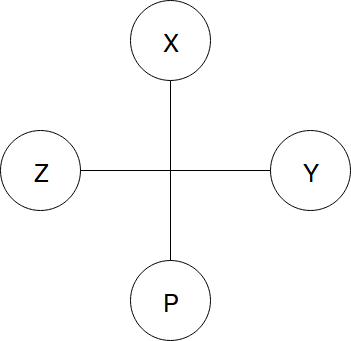
\includegraphics[width=0.32\textwidth]{softComb}
\caption{Vincolo risultante}
\end{figure}

\subsection{Ricerca di una soluzione con i vincoli soft}

Si visita ogni assegnamento che potrebbe essere una soluzione e si saltano
quelli che sono ``dominati'' da altri.

Ricerca branch and bound: si tiene traccia di un lower bound (preferenza
della migliore soluzione trovata) e di un upper bound (preferenza data dalle
variabili assegnate fino al nodo in cui ci si trova).

Il lower bound si inizializza con \textbf{l'elemento bottom del c-semianello}
utilizzato e viene aggiornato ogni volta che si incontra una soluzione
ammissibile migliorante a seconda del tipo di problema.

Se il problema è di minimizzazione e upper bound > lower bound (ho già una
soluzione migliore di quella che sto costruendo) si taglia il
sottoalbero, viceversa se il problema è di massimizzazione.

Se la soluzione non è feasible (non ci sono preferenze) allora
\textbf{non va considerata} nel branch and bound.
